\documentclass{article}

%package setup
\usepackage{graphicx}
\usepackage{amsmath}
\usepackage{fancyhdr}
\usepackage[margin=1in]{geometry}
\usepackage{comment}
\usepackage{placeins}
\usepackage{parskip}
\usepackage{subcaption}
\usepackage{appendix}
\usepackage{soul}
\usepackage{comment}
\usepackage[hidelinks]{hyperref}
\usepackage{matlab-prettifier}
\usepackage{minted}
\usepackage{enumitem}
\usepackage{float}
\usepackage{textcomp, gensymb}

\pagestyle{fancy}
\fancyhf{} % Clear header/footer settings
\rhead{\thepage} % Page number on the right in the header
\lhead{ASE375 Lab Report 4} % Your lab report title on the left

\begin{document}

\begin{titlepage}
  \centering
  
\includegraphics[width=10cm]{ase-logo-formal.png}  % Adjust the width as needed
  \vspace{1cm}  % Add some vertical space
 
  \Large \textbf{ASE 375 Electromechanical Systems}\\
  \large \textbf{Section 14115}\\
  \vspace{0.5cm}
  \textbf{Monday: 3:00 - 6:00 pm}\\
 
  \vspace{1cm}
 
  \hrule
  \vspace{0.5cm}
 
  \Huge \textbf{Report 4:\\
  Measuring Pressure Vessels}\\
  \Huge \textbf{}\\
 
  \vspace{0.5cm}
  \hrule
 
  \vspace{1cm}
 
  \normalsize \textbf{Andrew Doty, Andres Suniaga, Dennis Hom}\\
  \normalsize \textbf{Due Date: 02/26/2024}
 
\end{titlepage}
\newpage

\tableofcontents
\thispagestyle{empty}
\newpage

\section{Introduction}
In this experiment we (1) Learn how to measure pressure with different sensors, (2) Construct a Wheatstone quarter-bridge circuit, and (3) Develop an understanding for strain gauge measurements. 

In this two-part experiment we gather input voltage readings for the pressure of two vessels containing liquid using two different methods. The first method involves calibrated pressure transducers and a full strain gauge bridge with a direct application of pressure to the vessel. The second method involves constructing a quarter-bridge circuit to read strain measurements on a soda can as pressure is released. These demonstrations set a foundation for understanding the precision and sensitivity of these sensors used to measure pressure. 

\section{Equipment}
Devices used in this lab include:
\begin{itemize}

\item Digital Calipers: Used for measuring outer and inner dimensions of objects. In our case...
\vspace{2.5mm}

\item PX309 SERIES Pressure Transducer/Transmitter: Transducer used to read ...
\vspace{2.5mm}

\item Strain Gauge: Sensor used to ...
\vspace{2.5mm}

\item Cylindrical Poly-carbonate Vessel:...
\vspace{2.5mm}

\item Aluminum Soda Can: ... 
\vspace{2.5mm}

\item Pressure Regulator/Dial: 
\vspace{2.5mm}

\item DAQ, NI-9215 Voltage Input Module, and LabVIEW: Data Acquisition System used to process sample measurements into digital data. NI-9215 is an analog input used to measure the input voltage signals and send it through the DAQ system. LabVIEW used to model input voltages read from the DAQ of the transducer and strain gauge measurements.
\vspace{2.5mm}

\item Solderless Breadboard and Jumper Wires: Used to make connections ... 

\end{itemize}

\section{Procedure}

\section{Data Processing}

For part 1, our first values will be in voltages. We will convert these to pressures using the following equation:
\[
P = \frac{V}{0.004} - 14.7
\]

What are any of the sources of error or discrepancies in the data? How can we account for these?
- The gauge on the pressure vessel may not be accurate
- The true measurements were likely taken with an inaccurate gauge, and our uncertainties are likely larger than we think
- Over time, the pressure vessel leaked
- The pressure vessel could be at a different temperature than the room temperature
- The DAQ could be interpreting the data incorrectly from an error in the voltage.
- Delay in pressure changes from the valve opening.


\section{Results and Analysis}

\section{Conclusion}

\newpage
\thispagestyle{empty}  % Clear header/footer
\begin{center}
	\vspace*{\fill}
	{\Huge Appendices}
	\vspace*{\fill}
\end{center}

% Start appendices
\newpage
\begin{appendices}
\pagestyle{fancy}
\renewcommand{\thefigure}{A\arabic{figure}}
\setcounter{figure}{0}

\section*{Appendix: t-Distribution Tables}
\hypertarget{1}{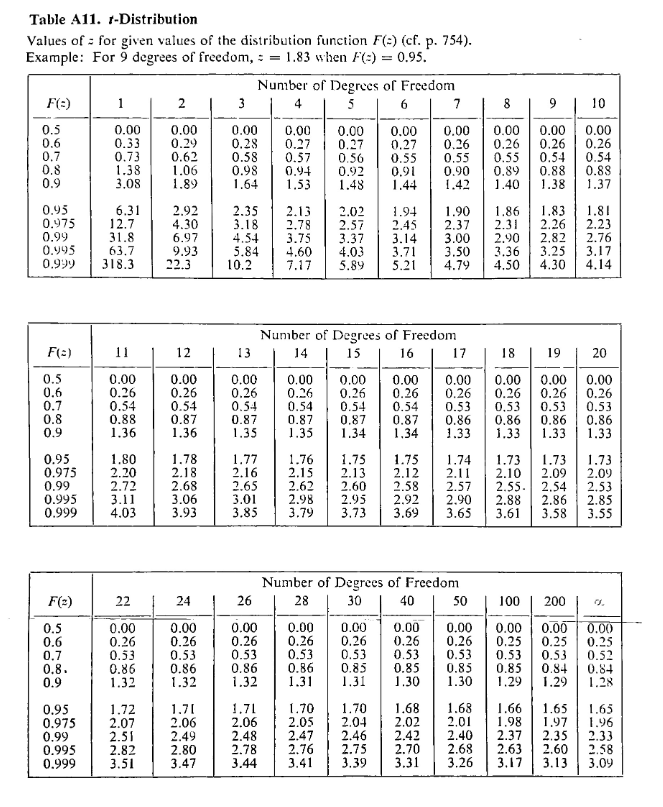
\includegraphics[width=0.95\textwidth]{t_distribution_Table_lecture3.png}}

\section*{Appendix: NI-9215 Datasheet}
\href{https://www.amc-systeme.de/files/pdf/ni-9215-amc.pdf}{NI-9215 Datasheet}
\end{appendices}

\end{document}
